\section{Diagramma delle Interfacce}
Il diagramma in \autoref{fig:IT1InterfaceDiagram} mostra le interfacce del sistema con le relative funzioni operative e i dati di input e output. La rappresentazione evidenzia inoltre la netta separazione dei livelli applicativi (layer) in conformità al design pattern architetturale Model-View-Controller (MVC).
\begin{figure}[H]
    \centering
    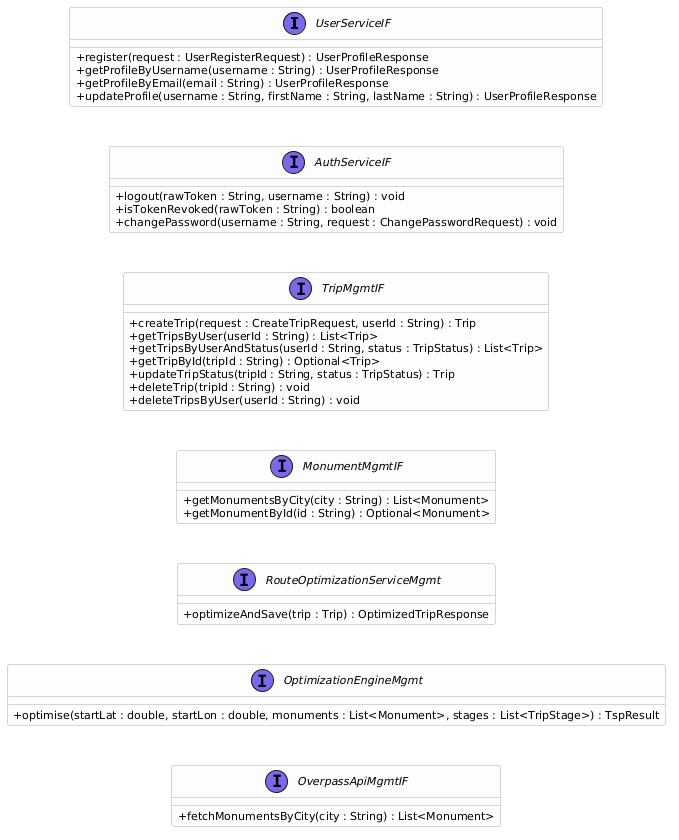
\includegraphics[width=0.75\textwidth]{Iterazione1/Diagrammi/InterfaceDiagram.png}
    \caption{Diagramma delle interfacce}
    \label{fig:IT1InterfaceDiagram}
\end{figure}    
